% Start - Hardware/Control Unit/MCU
%write Between the comments

\subsubsection{MCU}

	 \lettrine{T}{he} MCU is the central processing unit of the system. For this application/project the ATmega328P, by Atmel corporation, provides all the feature required. Following is the list of features \cite{AtMega328P}.
	 
	 \begin{itemize}
		\item Advanced RISC architecture
		\item 32K bytes of in-system self-programmable flash program memory.
		\item 1Kbytes EEPROM.
		\item 2Kbytes SRAM.
		\item Two 8-bit Timer/Counters
		\item One 16-bit Timer/Counter
		\item Six PWM channels
		\item 8-channel 10-bit ADC
		\item USART
		\item Master/slave SPI
		\item I2C
		\item watchdog timer
		\item On-chip analog comparator
		\item Six sleep modes 
		
		
	%	\begin{minipage}{0.3\textwidth}
	%		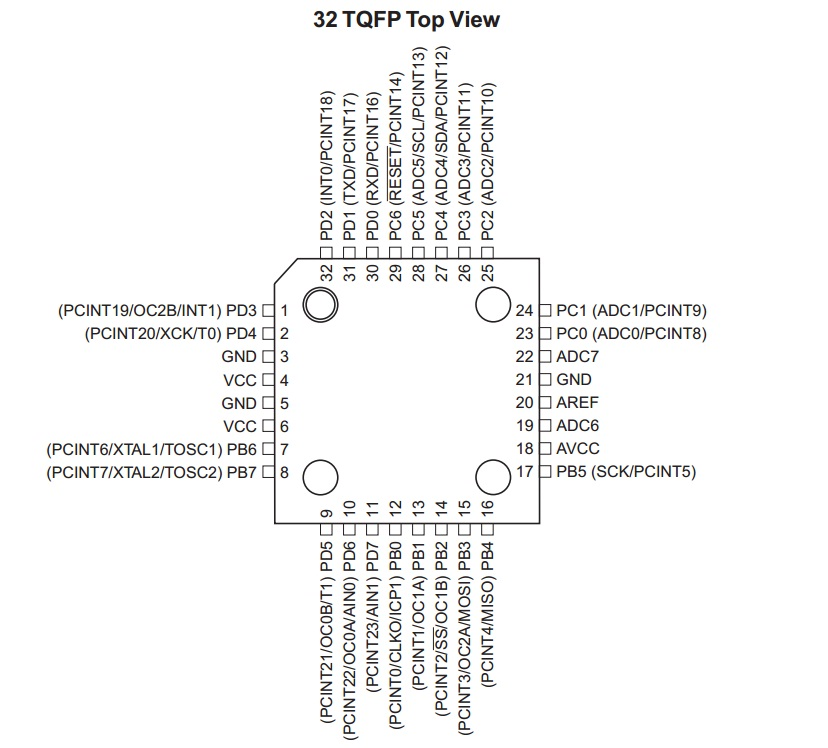
\includegraphics[width=\linewidth]{ATMega328p_TQFP_Pinout.jpg}
			%\caption{Block Diagram V0.21}
		%	\label{fig:image1}
			
		
		%\end{minipage}
		
	\end{itemize}	  
	 
	 

% End - Hardware/Control Unit/MCU
